\documentclass[../main.tex]{subfiles}
\graphicspath{{\subfix{../images/}}}
\begin{document}

\subsection{Pre-Processing}

Adapting what was used in the AlexNet Model, after images were sized, the images were cropped to include only the pixels in the center of the image.

In addition to this change, RandAugment in PyTorch can apply random changes to the images as they are loaded. With random augmentations, images could be oriented differently by flipping them vertically and horizontally, and rotated. The images could also be colored different such as increasing the contrast or saturation. 

\begin{figure}[h!]
  \centering
  \begin{subfigure}[b]{0.2\linewidth}
    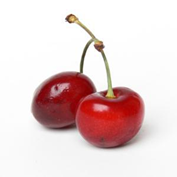
\includegraphics[width=\linewidth]{01-Contrast-Sharpness/original.png}
  \end{subfigure}
  \begin{subfigure}[b]{0.2\linewidth}
    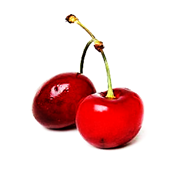
\includegraphics[width=\linewidth]{01-Contrast-Sharpness/edited.png}
  \end{subfigure}
  \caption{Cherry with increased contrast and sharpness}
  \label{fig:contrast-edit}
\end{figure}

\begin{figure}[h!]
  \centering
  \begin{subfigure}[b]{0.5\linewidth}
    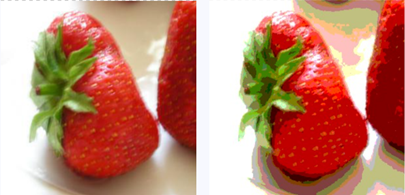
\includegraphics[width=\linewidth]{02-Posterising/strawberry.png}
  \end{subfigure}
  \caption{Strawberry Images with Posterising}
  \label{fig:strawberry-postering-edit}
\end{figure}

These changes trains the network to see a range of patterns that may not be obvious if all images were all the same. By learning these patterns from edited images, the network should improve its predictions for the unedited testing set. 

\begin{figure}[h!]
  \centering
  \begin{subfigure}[b]{0.35\linewidth}
    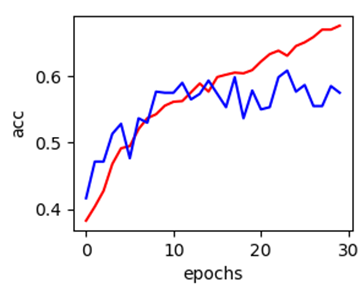
\includegraphics[width=\linewidth]{pre-processing-performance.png}
  \end{subfigure}
  \caption{Performance with Random Augmentation}
  \label{fig:preprocessing-performance}
\end{figure}

We see from Figure \ref{fig:preprocessing-performance} that our accuracy is between 55\% and 60\% which improves upon the previous model by about 5\%. 

\end{document}